\documentclass{standalone}
\usepackage{tikz}
\usetikzlibrary{patterns, positioning}

\begin{document}
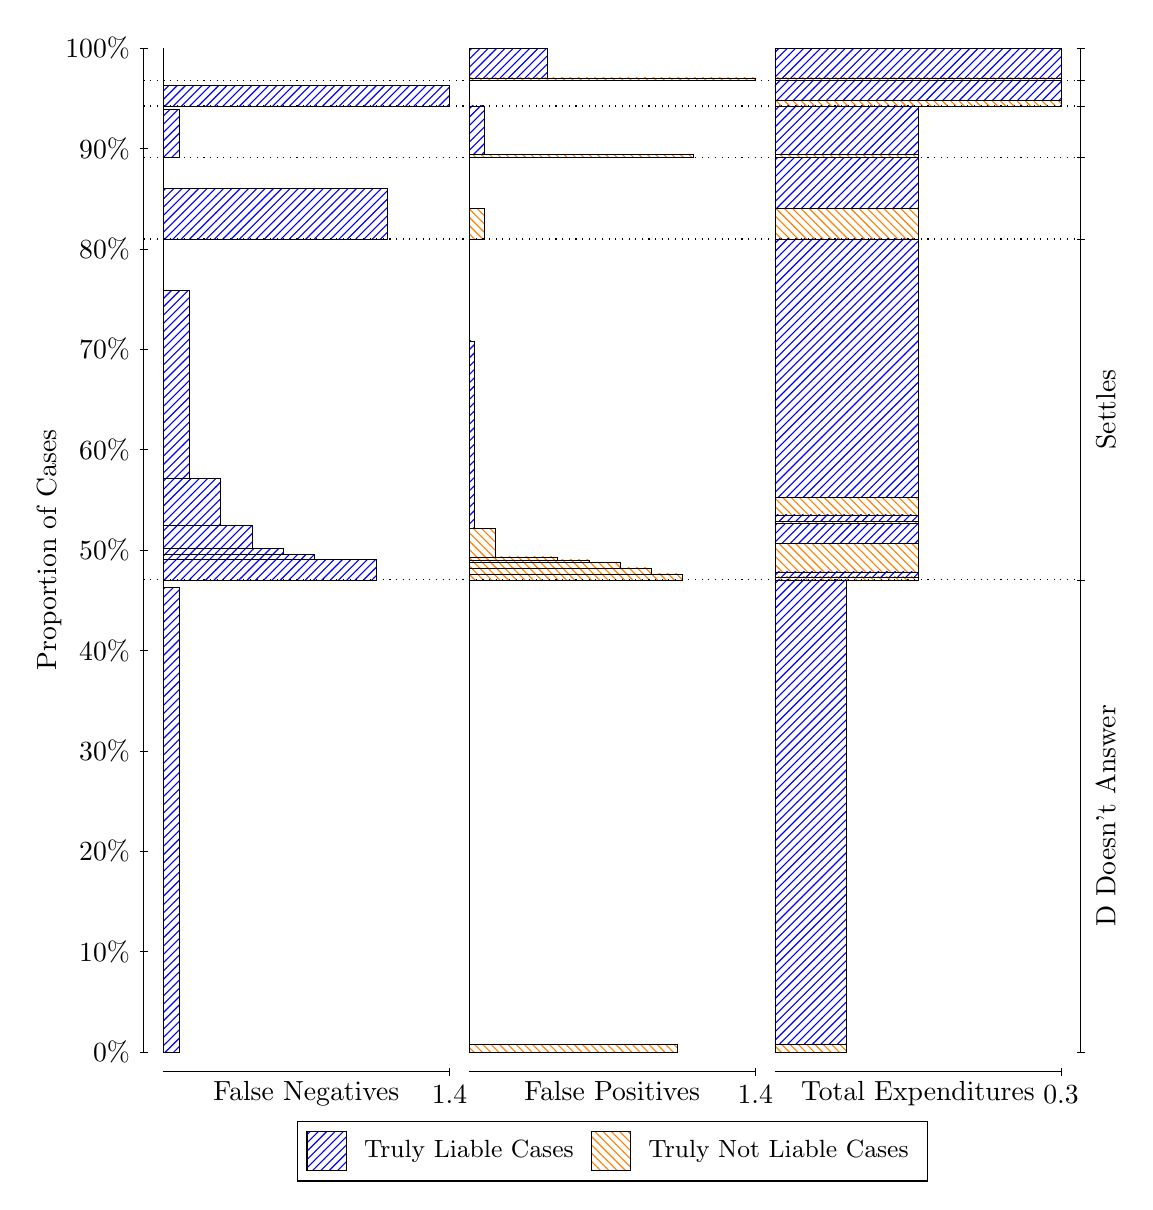
\begin{tikzpicture}
\draw[black, very thin] (1.5,1.75) -- (1.5,14.5);
\node[rotate=90, anchor=center] at (0.3, 8.125) {Proportion of Cases};
\draw[black, very thin] (1.45,1.75) -- (1.55,1.75);
\node[anchor=east] at (1.45, 1.75) {0\%};
\draw[black, very thin] (1.45,3.025) -- (1.55,3.025);
\node[anchor=east] at (1.45, 3.025) {10\%};
\draw[black, very thin] (1.45,4.3) -- (1.55,4.3);
\node[anchor=east] at (1.45, 4.3) {20\%};
\draw[black, very thin] (1.45,5.575) -- (1.55,5.575);
\node[anchor=east] at (1.45, 5.575) {30\%};
\draw[black, very thin] (1.45,6.85) -- (1.55,6.85);
\node[anchor=east] at (1.45, 6.85) {40\%};
\draw[black, very thin] (1.45,8.125) -- (1.55,8.125);
\node[anchor=east] at (1.45, 8.125) {50\%};
\draw[black, very thin] (1.45,9.4) -- (1.55,9.4);
\node[anchor=east] at (1.45, 9.4) {60\%};
\draw[black, very thin] (1.45,10.675) -- (1.55,10.675);
\node[anchor=east] at (1.45, 10.675) {70\%};
\draw[black, very thin] (1.45,11.95) -- (1.55,11.95);
\node[anchor=east] at (1.45, 11.95) {80\%};
\draw[black, very thin] (1.45,13.225) -- (1.55,13.225);
\node[anchor=east] at (1.45, 13.225) {90\%};
\draw[black, very thin] (1.45,14.5) -- (1.55,14.5);
\node[anchor=east] at (1.45, 14.5) {100\%};

\draw[black, very thin] (13.4,1.75) -- (13.4,14.5);
\draw[black, very thin] (13.35,1.75) -- (13.45,1.75);
\node[anchor=west] at (13.35, 1.75) {};
\draw[black, very thin] (13.35,7.7461) -- (13.45,7.7461);
\node[anchor=west] at (13.35, 7.7461) {};
\draw[black, very thin] (13.35,12.075) -- (13.45,12.075);
\node[anchor=west] at (13.35, 12.075) {};
\draw[black, very thin] (13.35,13.109) -- (13.45,13.109);
\node[anchor=west] at (13.35, 13.109) {};
\draw[black, very thin] (13.35,13.764) -- (13.45,13.764);
\node[anchor=west] at (13.35, 13.764) {};
\draw[black, very thin] (13.35,14.092) -- (13.45,14.092);
\node[anchor=west] at (13.35, 14.092) {};
\draw[black, very thin] (13.35,14.5) -- (13.45,14.5);
\node[anchor=west] at (13.35, 14.5) {};

\draw[black, very thin, pattern color=blue, pattern=north east lines] (1.75,1.75) rectangle (1.9482,7.6492);
\draw[black, very thin, pattern color=orange, pattern=north west lines] (1.75,7.6492) rectangle (1.75,7.7461);
\draw[black, very thin, pattern color=blue, pattern=north east lines] (1.75,7.7461) rectangle (4.4585,8.004);
\draw[black, very thin, pattern color=blue, pattern=north east lines] (1.75,8.004) rectangle (3.6658,8.0656);
\draw[black, very thin, pattern color=blue, pattern=north east lines] (1.75,8.0656) rectangle (3.2694,8.1452);
\draw[black, very thin, pattern color=blue, pattern=north east lines] (1.75,8.1452) rectangle (2.873,8.4401);
\draw[black, very thin, pattern color=blue, pattern=north east lines] (1.75,8.4401) rectangle (2.4767,9.0394);
\draw[black, very thin, pattern color=blue, pattern=north east lines] (1.75,9.0394) rectangle (2.0803,11.425);
\draw[black, very thin, pattern color=orange, pattern=north west lines] (1.75,11.425) rectangle (1.75,12.075);
\draw[black, very thin, pattern color=blue, pattern=north east lines] (1.75,12.075) rectangle (4.5906,12.721);
\draw[black, very thin, pattern color=orange, pattern=north west lines] (1.75,12.721) rectangle (1.75,13.109);
\draw[black, very thin, pattern color=blue, pattern=north east lines] (1.75,13.109) rectangle (1.9482,13.725);
\draw[black, very thin, pattern color=orange, pattern=north west lines] (1.75,13.725) rectangle (1.75,13.764);
\draw[black, very thin, pattern color=blue, pattern=north east lines] (1.75,13.764) rectangle (5.3833,14.021);
\draw[black, very thin, pattern color=orange, pattern=north west lines] (1.75,14.021) rectangle (1.75,14.092);
\draw[black, very thin, pattern color=orange, pattern=north west lines] (1.75,14.092) rectangle (1.75,14.12);
\draw[black, very thin, pattern color=blue, pattern=north east lines] (1.75,14.12) rectangle (1.75,14.5);
\draw[black, very thin, pattern color=orange, pattern=north west lines] (5.6333,1.75) rectangle (8.2758,1.8469);
\draw[black, very thin, pattern color=blue, pattern=north east lines] (5.6333,1.8469) rectangle (5.6333,7.7461);
\draw[black, very thin, pattern color=orange, pattern=north west lines] (5.6333,7.7461) rectangle (8.3418,7.8214);
\draw[black, very thin, pattern color=orange, pattern=north west lines] (5.6333,7.8214) rectangle (7.9455,7.899);
\draw[black, very thin, pattern color=orange, pattern=north west lines] (5.6333,7.899) rectangle (7.5491,7.9697);
\draw[black, very thin, pattern color=orange, pattern=north west lines] (5.6333,7.9697) rectangle (7.1527,7.9989);
\draw[black, very thin, pattern color=orange, pattern=north west lines] (5.6333,7.9989) rectangle (6.7564,8.0375);
\draw[black, very thin, pattern color=orange, pattern=north west lines] (5.6333,8.0375) rectangle (5.9636,8.3962);
\draw[black, very thin, pattern color=blue, pattern=north east lines] (5.6333,8.3962) rectangle (5.6994,10.782);
\draw[black, very thin, pattern color=blue, pattern=north east lines] (5.6333,10.782) rectangle (5.6333,12.075);
\draw[black, very thin, pattern color=orange, pattern=north west lines] (5.6333,12.075) rectangle (5.8315,12.464);
\draw[black, very thin, pattern color=blue, pattern=north east lines] (5.6333,12.464) rectangle (5.6333,13.109);
\draw[black, very thin, pattern color=orange, pattern=north west lines] (5.6333,13.109) rectangle (8.4739,13.149);
\draw[black, very thin, pattern color=blue, pattern=north east lines] (5.6333,13.149) rectangle (5.8315,13.764);
\draw[black, very thin, pattern color=orange, pattern=north west lines] (5.6333,13.764) rectangle (5.6333,13.835);
\draw[black, very thin, pattern color=blue, pattern=north east lines] (5.6333,13.835) rectangle (5.6333,14.092);
\draw[black, very thin, pattern color=orange, pattern=north west lines] (5.6333,14.092) rectangle (9.2667,14.12);
\draw[black, very thin, pattern color=blue, pattern=north east lines] (5.6333,14.12) rectangle (6.6242,14.5);
\draw[black, very thin, pattern color=orange, pattern=north west lines] (9.5167,1.75) rectangle (10.425,1.8469);
\draw[black, very thin, pattern color=blue, pattern=north east lines] (9.5167,1.8469) rectangle (10.425,7.7461);
\draw[black, very thin, pattern color=orange, pattern=north west lines] (9.5167,7.7461) rectangle (11.333,7.7847);
\draw[black, very thin, pattern color=blue, pattern=north east lines] (9.5167,7.7847) rectangle (11.333,7.8463);
\draw[black, very thin, pattern color=orange, pattern=north west lines] (9.5167,7.8463) rectangle (11.333,8.205);
\draw[black, very thin, pattern color=blue, pattern=north east lines] (9.5167,8.205) rectangle (11.333,8.4629);
\draw[black, very thin, pattern color=orange, pattern=north west lines] (9.5167,8.4629) rectangle (11.333,8.4921);
\draw[black, very thin, pattern color=blue, pattern=north east lines] (9.5167,8.4921) rectangle (11.333,8.5717);
\draw[black, very thin, pattern color=orange, pattern=north west lines] (9.5167,8.5717) rectangle (11.333,8.7953);
\draw[black, very thin, pattern color=blue, pattern=north east lines] (9.5167,8.7953) rectangle (11.333,12.075);
\draw[black, very thin, pattern color=orange, pattern=north west lines] (9.5167,12.075) rectangle (11.333,12.464);
\draw[black, very thin, pattern color=blue, pattern=north east lines] (9.5167,12.464) rectangle (11.333,13.109);
\draw[black, very thin, pattern color=orange, pattern=north west lines] (9.5167,13.109) rectangle (11.333,13.149);
\draw[black, very thin, pattern color=blue, pattern=north east lines] (9.5167,13.149) rectangle (11.333,13.764);
\draw[black, very thin, pattern color=orange, pattern=north west lines] (9.5167,13.764) rectangle (13.15,13.835);
\draw[black, very thin, pattern color=blue, pattern=north east lines] (9.5167,13.835) rectangle (13.15,14.092);
\draw[black, very thin, pattern color=orange, pattern=north west lines] (9.5167,14.092) rectangle (13.15,14.12);
\draw[black, very thin, pattern color=blue, pattern=north east lines] (9.5167,14.12) rectangle (13.15,14.5);
\draw[black, dotted] (1.5,7.7461) -- (13.4,7.7461);
\draw[black, dotted] (1.5,12.075) -- (13.4,12.075);
\draw[black, dotted] (1.5,13.109) -- (13.4,13.109);
\draw[black, dotted] (1.5,13.764) -- (13.4,13.764);
\draw[black, dotted] (1.5,14.092) -- (13.4,14.092);
\draw[black, very thin] (1.75,1.5) -- (5.3833,1.5);
\node[anchor=north] at (3.5667, 1.5) {False Negatives};
\draw[black, very thin] (5.3833,1.45) -- (5.3833,1.55);
\node[anchor=north] at (5.3833, 1.45) {1.4};

\draw[black, very thin] (5.6333,1.5) -- (9.2667,1.5);
\node[anchor=north] at (7.45, 1.5) {False Positives};
\draw[black, very thin] (9.2667,1.45) -- (9.2667,1.55);
\node[anchor=north] at (9.2667, 1.45) {1.4};

\draw[black, very thin] (9.5167,1.5) -- (13.15,1.5);
\node[anchor=north] at (11.333, 1.5) {Total Expenditures};
\draw[black, very thin] (13.15,1.45) -- (13.15,1.55);
\node[anchor=north] at (13.15, 1.45) {0.3};

\node[black, centered, rotate=90] at (13.72, 4.748) {D Doesn't Answer};
\node[black, centered, rotate=90] at (13.72, 9.9106) {Settles};





\draw (7.449999999999999,1.5) node[draw=none] (baseCoordinate) {};
\begin{scope}[align=center]
        \matrix[scale=0.5, draw=black, below=0.5cm of baseCoordinate, nodes={draw}, column sep=0.1cm]{
            \node[rectangle, draw, minimum width=0.5cm, minimum height=0.5cm, pattern=north east lines, pattern color=blue] {}; &
            \node[draw=none, font=\small] (B) {Truly Liable Cases}; &
            \node[rectangle, draw, minimum width=0.5cm, minimum height=0.5cm, pattern=north west lines, pattern color=orange] {}; &
            \node[draw=none, font=\small] (B) {Truly Not Liable Cases}; \\
            };
\end{scope}

\end{tikzpicture}
\end{document}